\subsection{Experiment results – effects of parameters}
\label{section:distributions-results-trends}

Figure \ref{fig:dimension} illustrates how the performance of outlierness measures is affected by the dimension of the feature vectors $d$, under fixed number of training samples $n = 2500$ and distance to outliers $h = 8$. The experiments shows that higher the feature space dimension $d$, the more challenging the comparison between data vectors is, as both classification accuracy and AUROC score decrease. The research was focused on ED, IRWD, kNN, LOF, MD and SED measures, omitting ABOF as computationally too expensive and impractical for usage (primarily due to $n$; although it was reaching promising top-scores for lower $n$ and $d$).

All of the analyzed measures $OF$ provide good separability of in-distribution data and outliers in lower dimensions – reaching AUROC value above $0.95$ for $d \leq 200$. In higher dimensions, the outliers distribution appear closer to the training data, so the obtained AUROC values are lower, decreasing exponentially with $d$. For dimension $d = 1000$ the AUROC reaches about ${\sim}0.85$ in case of ED and SED (plots overlap in figure \ref{fig:dimension-auroc}), ${\sim}0.84$ for kNN and LOF, ${\sim}0.78$ for MD and ${\sim}0.715$ in case of IRWD (results visible in subfigure \ref{fig:dimension-auroc}).

Although offering good separability, when the measures are involved in the classification task with respect to the training data only, not all $OF$s perform so well. Notably the kNN's performance falls drastically, reaching accuracy of ${\sim}0.5$ for $d \geq 250$. Similarly, the MD measure, after initially performing well ($d \leq 250$), shows gradual decay of accuracy in higher dimensions ($d \geq 500$). In both mentioned cases it is related to the lose of sensitivity, as visible in figure \ref{fig:dimension-sensitivity} – at some point all in-distribution data were recognized as outliers by kNN and MD (due to the same effect discussed in previous subsection \ref{section:distributions-results-properties} and visible in figure \ref{fig:hists-dimensions}).
% This is significant because, in the real-world scenario, where we would not know where the outliers are distributed, our OOD detection threshold should only rely on the distribution of the available training set. However, as shown in this example, this may lead to poor classification accuracy, as accuracy finally drops to 50\% (i.e., all data are classified as outliers).
% TODO \todo{significant}

Contrary, in case of ED, SED, IRWD and LOF the lowered accuracy in high-dimensions is related purely to the decaying specificity – some out-of-distribution data are seen as too close to the training data, such as in histograms in previous subsection \ref{section:distributions-results-properties} (subfigures \ref{fig:histogram-euclidean}, \ref{fig:histogram-irwd} and \ref{fig:histogram-lof}), hence spuriously considered as inliers.

Figure \ref{fig:samples} shows analogous research, analyzing the performance of outlierness measures $OF$ affected by the number of training samples $n$, having fixed dimension of the feature vectors $d = 750$ and distance to outliers $h = 8$. Surprisingly, no strong influence between the accuracy and separability (AUROC value) is observed – except for extremely underrepresented cases ($n < 100$ for $d = 750$, not show in the figure) or~Mahalanobis Distance measure.

The estimation of covariance matrix for MD in features space of dimension $d = 750$ requires at least $n \geq 750$ data samples. Hence, first reasonable result for MD visible in figure \ref{fig:samples-auroc} appears for $n = 1000$ –~AUROC value ${\sim}0.715$; for $n = 750$ samples the AUROC is ${\sim}0.5$. For $n = 10000$ samples the reaches close to top AUROC score ${\sim}0.85$.

The best separability in analyzed case is again observed for ED and SED measures (AUROC values ${\sim}0.86$), then kNN and LOF (AUROC values ${\sim}0.85$). The IRWD performed significantly worse, scoring AUROC value ${\sim}0.76$. Similarly like in previously examined case, the good AUROC score does not translate to good accuracy in the classification task with respect to the training data. Again, it is due to the zero TPR score (sensitivity) – all in-distribution data are incorrectly recognized as outliers, because the outlierness scores for testing set do not overlap the scores for training set (as visible in figure \ref{fig:hists-dimensions}). In case of MD, low accuracy is observed for up to $n \leq 2500$ samples, because of the same effect as for kNN, however by providing more training samples ($n \geq 5000$) the scores for in-distribution testing samples start to overlap with scores for training samples (effect visible in figure \ref{fig:hists-md-samples}), in the end obtaining one of the top accuracy for $n = 10000$. Yet, ED, SED and LOF reach similar accuracy for lower number of training samples $n$.

Finally, figure \ref{fig:distance} presents the performance of outlierness measures $OF$ as affected by the distance to outliers $h$, under fixed dimension of the feature vectors $d = 750$ and number of training samples $n = 2500$. Intuitively, the more distant the outliers are, the easier they are separable and detectable, like discussed in section \ref{section:near-far-ood} (Near OOD vs Far OOD). The relation is analogous as in first analyzed case – resulting in best separability for ED, SED, kNN and LOF, then for MD and worst for IRWD under given experiment configuration. Again, the worst possible accuracy is observed for kNN and MD, as for given $n$ and $d$ all the data are recognized as outliers (zero sensitivity). The ED, SED, IRWD and LOF initially do not recognize any outliers (zero specificity), until they are significantly distant $h > 4$.

The experiments were repeated for various distributions generators ($Gaussian$, $Triangular$, $Uniform$), however no significant differences were observed – both the classification and separability is easier (i.e., higher scores obtained) for a given set of parameters in case of the distributions with finite output domain ($G = Triangular$, $G = Uniform$), due to outliers appearing more distant, as seen in figure \ref{fig:histograms-other-G}, however the overall trends and behaviors of measures remain similar. Hence, only the results for $G = Gaussian$ distribution are presented in this section. Additionally it will make it easier comparable with following results in sections \ref{section:correlations-experiment} and \ref{section:variances-experiment}. All omitted results can be analyzed in the tooling described in appendix \ref{chapter:source-code}.

\begin{figure}[t]
    % Query: dimension >= 10 and dimension <= 1000
    \centering
    \begin{subfigure}[b]{0.9\textwidth}
        % StreamLit settings: width=9, height=4
        % X: [0.00, 1010.00]
        % Y: [0.69, 1.01]
        \centering
        \caption{\small Separability between in-distribution and out-of-distribution data}
        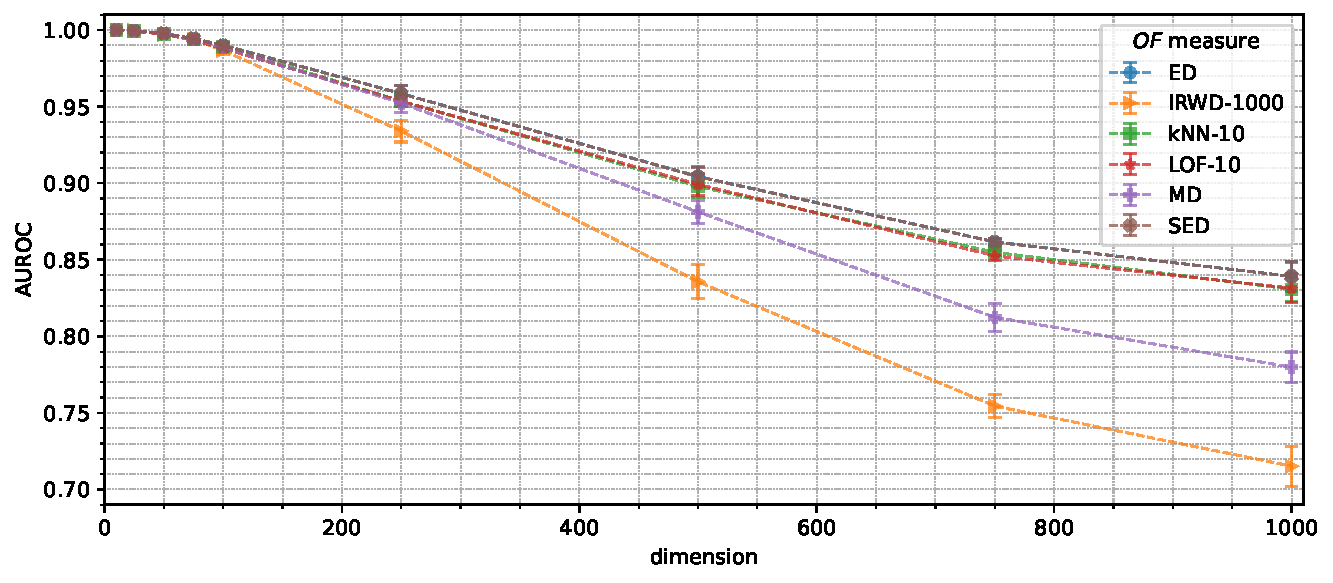
\includegraphics[width=\textwidth]{images/distributions/trends-d/trend-distributions-auroc(dimension)-samples_2500-distance_8-distribution_gaussian-model_ED,IRWD-1000,kNN-10,LOF-10,MD,SED-aggregated.pdf}
        \label{fig:dimension-auroc}
    \end{subfigure}
    \begin{subfigure}[b]{0.9\textwidth}
        % StreamLit settings: width=9, height=4
        % X: [0.00, 1010.00]
        % Y: [0.48, 1.00]
        \centering
        \caption{\small Classification with respect to the training data}
        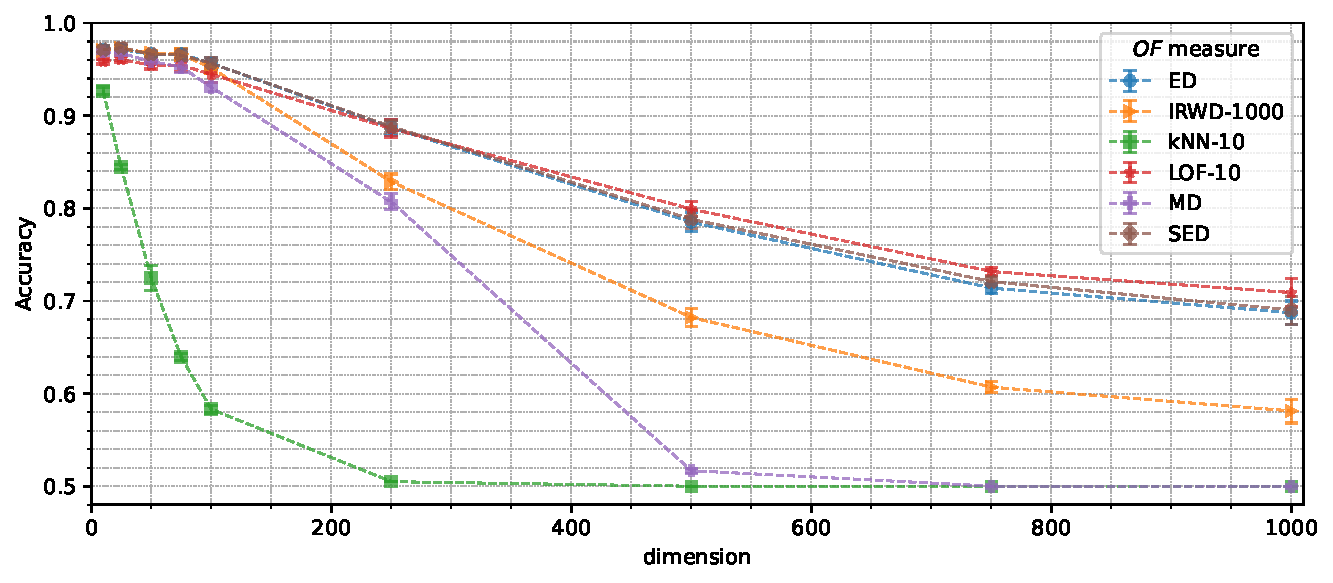
\includegraphics[width=\textwidth]{images/distributions/trends-d/trend-distributions-accuracy_95(dimension)-samples_2500-distance_8-distribution_gaussian-model_ED,IRWD-1000,kNN-10,LOF-10,MD,SED-aggregated.pdf}
        \label{fig:dimension-accuracy}
    \end{subfigure}
    \begin{subfigure}[b]{0.495\textwidth}
        % StreamLit settings: width=5, height=3
        % X: [0.00, 1010.00]
        % Y: [-0.02, 1.05]
        \centering
        \caption{\small Correctly recognized in-distribution}
        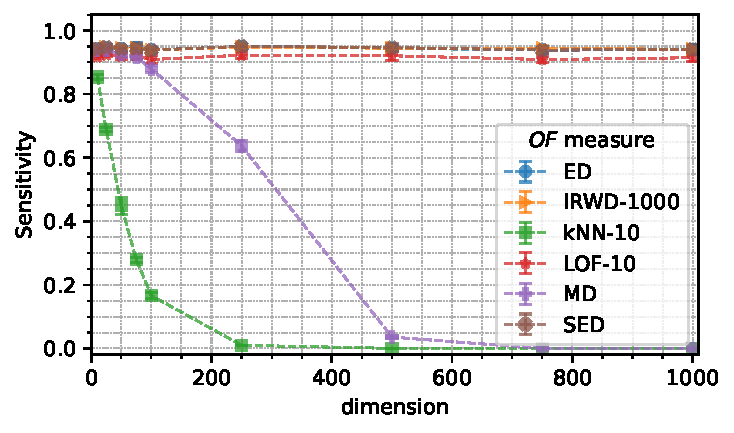
\includegraphics[width=\textwidth]{images/distributions/trends-d/trend-distributions-sens_95(dimension)-samples_2500-distance_8-distribution_gaussian-model_ED,IRWD-1000,kNN-10,LOF-10,MD,SED-aggregated.pdf}
        \label{fig:dimension-sensitivity}
    \end{subfigure}
    \hfill
    \begin{subfigure}[b]{0.495\textwidth}
        % StreamLit settings: width=5, height=3
        % X: [0.00, 1010.00]
        % Y: [-0.02, 1.05]
        \centering
        \caption{\small Correctly recognized out-of-distribution}
        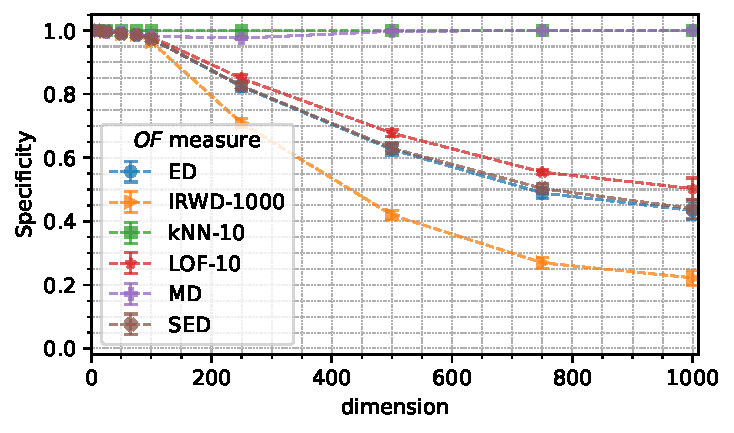
\includegraphics[width=\textwidth]{images/distributions/trends-d/trend-distributions-spec_95(dimension)-samples_2500-distance_8-distribution_gaussian-model_ED,IRWD-1000,kNN-10,LOF-10,MD,SED-aggregated.pdf}
        \label{fig:dimension-specificity}
    \end{subfigure}
    \caption{The performance of outlierness measures $OF$ as affected by the dimension of  the feature space $d$. The fixed parameters in the experiment are: number~of~training samples $n = 2500$, distance to outliers $h = 8$ and distribution $G = Gaussian$. The~results are aggregated for multiple generator seeds $\xi$ and~displayed as averages with~error~bars (standard deviation).}
    \label{fig:dimension}
    \vspace{-1.0em}
\end{figure}

\begin{figure}[t]
    % Query: samples >= 100 and samples <= 10000
    \centering
    \begin{subfigure}[b]{0.9\textwidth}
        % StreamLit settings: width=9, height=4
        % X: [95.00, 10500.00]
        % Y: [0.68, 0.88]
        \centering
        \caption{\small Separability between in-distribution and out-of-distribution data}
        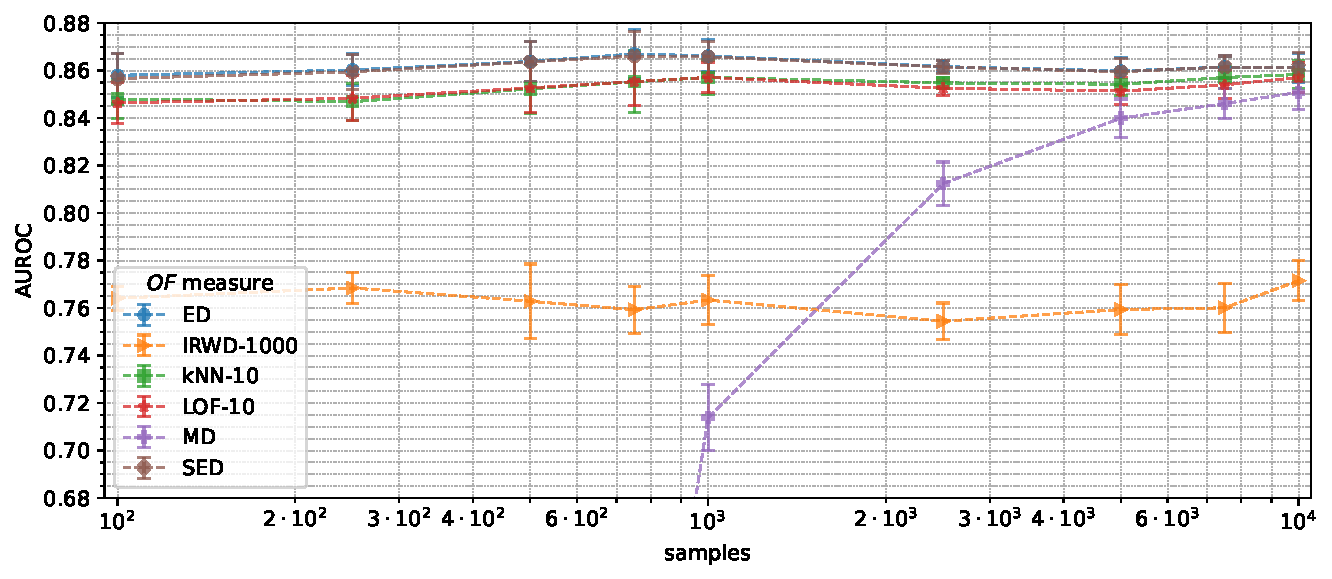
\includegraphics[width=\textwidth]{images/distributions/trends-n/trend-distributions-auroc(samples)-dimension_750-distance_8-distribution_gaussian-model_ED,IRWD-1000,kNN-10,LOF-10,MD,SED-aggregated.pdf}
        \label{fig:samples-auroc}
    \end{subfigure}
    \begin{subfigure}[b]{0.9\textwidth}
        % StreamLit settings: width=9, height=4
        % X: [95.00, 10500.00]
        % Y: [0,49, 0.80]
        \centering
        \caption{\small Classification with respect to the training data}
        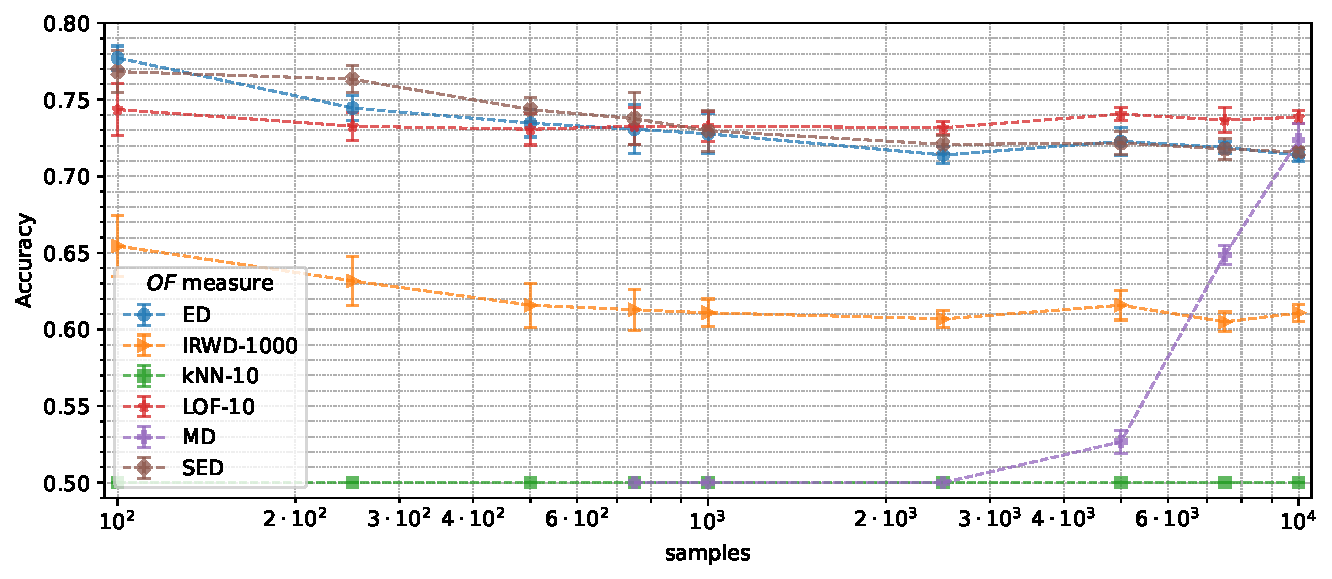
\includegraphics[width=\textwidth]{images/distributions/trends-n/trend-distributions-accuracy_95(samples)-dimension_750-distance_8-distribution_gaussian-model_ED,IRWD-1000,kNN-10,LOF-10,MD,SED-aggregated.pdf}
        \label{fig:samples-accuracy}
    \end{subfigure}
    \begin{subfigure}[b]{0.495\textwidth}
        % StreamLit settings: width=5, height=3
        % X: [95.00, 10500.00]
        % Y: [-0.02, 1.05]
        \centering
        \caption{\small Correctly recognized in-distribution}
        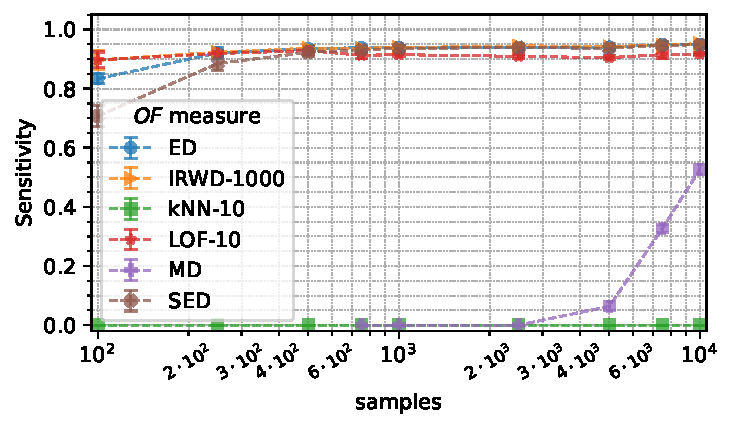
\includegraphics[width=\textwidth]{images/distributions/trends-n/trend-distributions-sens_95(samples)-dimension_750-distance_8-distribution_gaussian-model_ED,IRWD-1000,kNN-10,LOF-10,MD,SED-aggregated.pdf}
        \label{fig:samples-sensitivity}
    \end{subfigure}
    \hfill
    \begin{subfigure}[b]{0.495\textwidth}
        % StreamLit settings: width=5, height=3
        % X: [95.00, 10500.00]
        % Y: [-0.02, 1.05]
        \centering
        \caption{\small Correctly recognized out-of-distribution}
        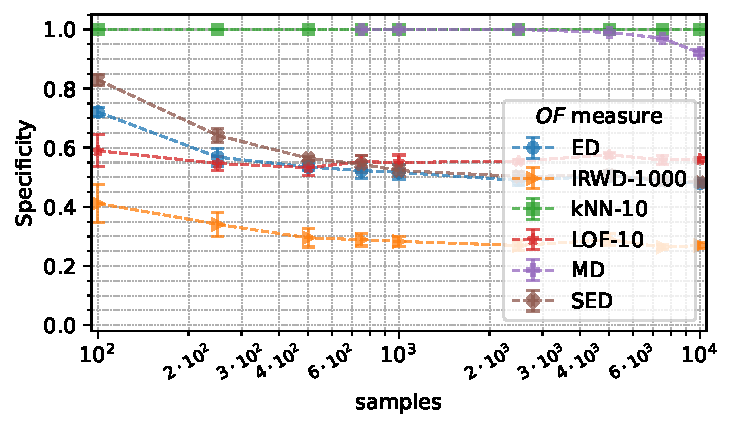
\includegraphics[width=\textwidth]{images/distributions/trends-n/trend-distributions-spec_95(samples)-dimension_750-distance_8-distribution_gaussian-model_ED,IRWD-1000,kNN-10,LOF-10,MD,SED-aggregated.pdf}
        \label{fig:samples-specificity}
    \end{subfigure}
    \caption{The performance of outlierness measures $OF$ as affected by the number of training samples $n$. The fixed parameters in the experiment are: dimension of the~feature space $d = 750$, distance to outliers $h = 8$ and distribution $G = Gaussian$. The~results are aggregated for multiple generator seeds $\xi$ and displayed as averages with~error~bars (standard deviation).}
    \label{fig:samples}
    \vspace{-1.0em}
\end{figure}

\begin{figure}[t]
    \centering
    \begin{subfigure}[b]{0.9\textwidth}
        % StreamLit settings: width=9, height=4
        % X: [0.96, 16.60]
        % Y: [0.46, 1.02]
        \centering
        \caption{\small Separability between in-distribution and out-of-distribution data}
        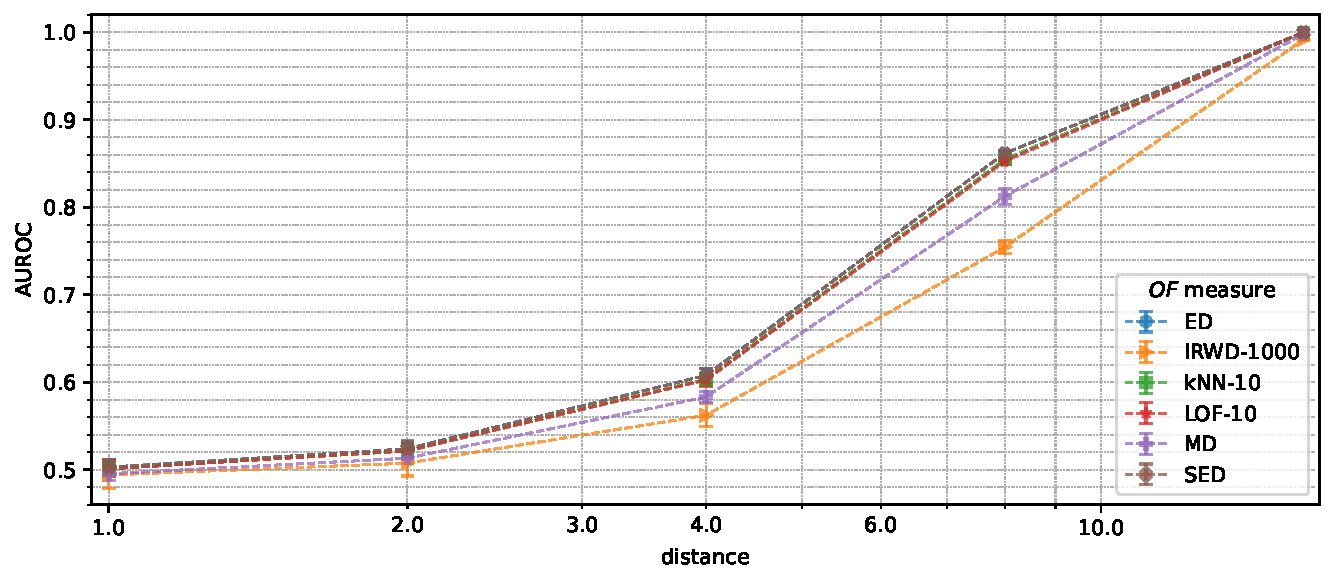
\includegraphics[width=\textwidth]{images/distributions/trends-h/trend-distributions-auroc(distance)-dimension_750-samples_2500-distribution_gaussian-model_ED,IRWD-1000,kNN-10,LOF-10,MD,SED-aggregated.pdf}
        \label{fig:distance-auroc}
    \end{subfigure}
    \begin{subfigure}[b]{0.9\textwidth}
        % StreamLit settings: width=9, height=4
        % X: [0.96, 16.60]
        % Y: [0,48, 1.00]
        \centering
        \caption{\small Classification with respect to the training data}
        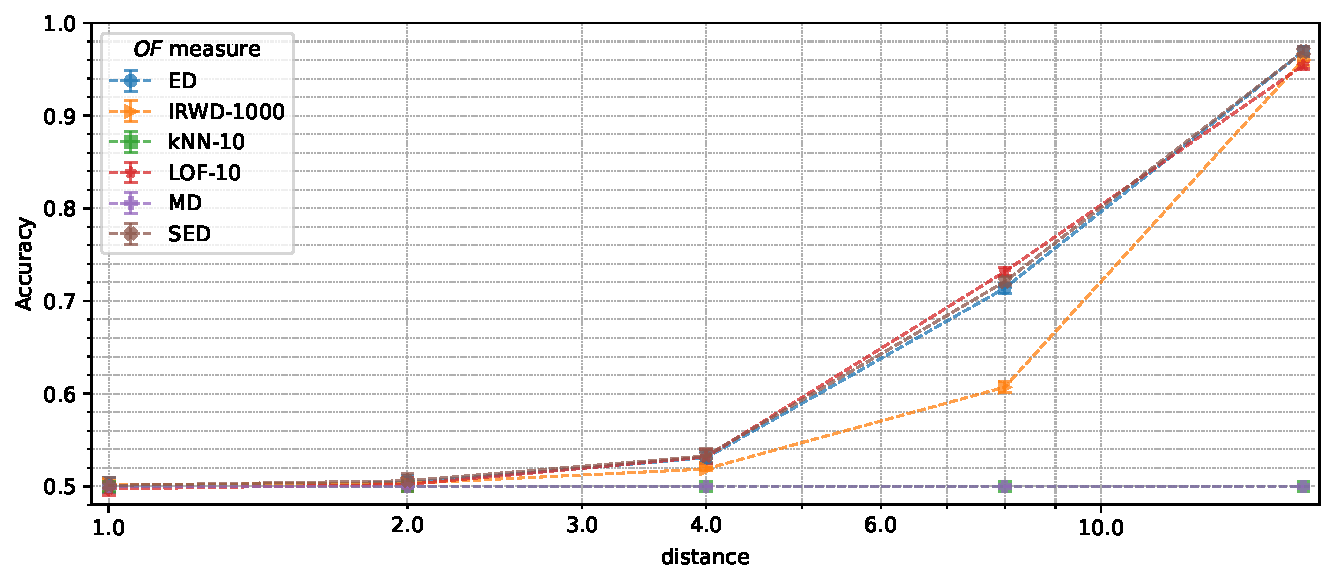
\includegraphics[width=\textwidth]{images/distributions/trends-h/trend-distributions-accuracy_95(distance)-dimension_750-samples_2500-distribution_gaussian-model_ED,IRWD-1000,kNN-10,LOF-10,MD,SED-aggregated.pdf}
        \label{fig:distance-accuracy}
    \end{subfigure}
    \begin{subfigure}[b]{0.495\textwidth}
        % StreamLit settings: width=5, height=3
        % X: [0.96, 16.60]
        % Y: [-0.02, 1.05]
        \centering
        \caption{\small Correctly recognized in-distribution}
        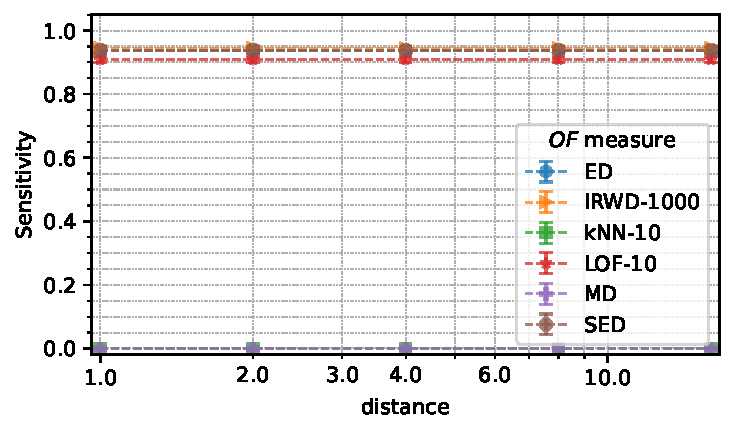
\includegraphics[width=\textwidth]{images/distributions/trends-h/trend-distributions-sens_95(distance)-dimension_750-samples_2500-distribution_gaussian-model_ED,IRWD-1000,kNN-10,LOF-10,MD,SED-aggregated (1).pdf}
        \label{fig:distance-sensitivity}
    \end{subfigure}
    \hfill
    \begin{subfigure}[b]{0.495\textwidth}
        % StreamLit settings: width=5, height=3
        % X: [0.96, 16.60]
        % Y: [-0.02, 1.05]
        \centering
        \caption{\small Correctly recognized out-of-distribution}
        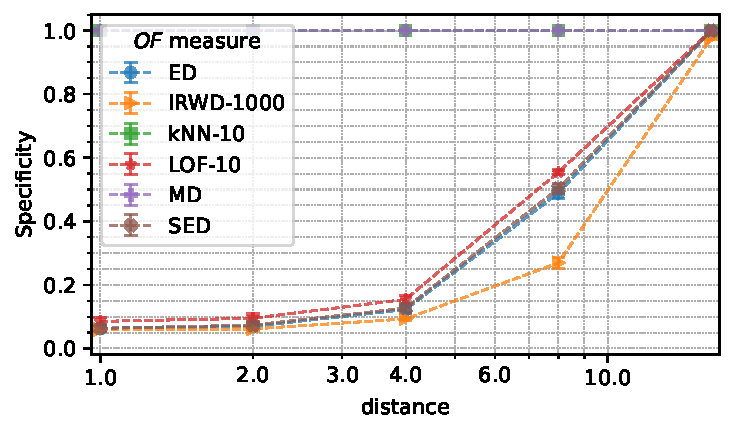
\includegraphics[width=\textwidth]{images/distributions/trends-h/trend-distributions-spec_95(distance)-dimension_750-samples_2500-distribution_gaussian-model_ED,IRWD-1000,kNN-10,LOF-10,MD,SED-aggregated.pdf}
        \label{fig:distance-specificity}
    \end{subfigure}
    \caption{The performance of outlierness measures $OF$ as affected by the distance to outliers $h$. The fixed parameters in the experiment are: dimension of the~feature space $d = 750$, number of training samples $n = 2500$ and distribution $G = Gaussian$. The~results are aggregated for multiple generator seeds $\xi$ and displayed as averages with~error~bars (standard deviation).}
    \label{fig:distance}
    \vspace{-1.0em}
\end{figure}

\cleardoublepage{}
